\documentclass[12pt]{article}
\usepackage[margin=1in]{geometry}
\usepackage{titlesec}
\usepackage{parskip}
\usepackage{listings}
\usepackage{xcolor}
\usepackage{hyperref}
\usepackage[T1]{fontenc}
\usepackage{pagecolor}
\usepackage{graphicx}
\usepackage{float}

% Dark theme colors
\definecolor{darkbg}{HTML}{121212}
\definecolor{lighttext}{HTML}{E6E6E6}
\definecolor{codegray}{HTML}{2D2D2D}
\definecolor{accent}{HTML}{8DA0B6}

% Set page and text colors
\pagecolor{darkbg}
\color{lighttext}

% Configure hyperref for dark background
\hypersetup{
    colorlinks=true,
    linkcolor=accent,
    filecolor=accent,
    urlcolor=accent,
    citecolor=accent,
}

% Title formatting
\titleformat{\section}{\centering\Large\bfseries\color{accent}}{\thesection}{1em}{}
\titleformat{\subsection}{\large\bfseries\color{accent}}{\thesubsection}{1em}{}

% Code listing style
\lstset{
    backgroundcolor=\color{codegray},
    basicstyle=\ttfamily\footnotesize\color{lighttext},
    frame=single,
    breaklines=true,
    postbreak=\mbox{\textcolor{accent}{$\hookrightarrow$}\space},
    rulecolor=\color{accent},
}

\begin{document}

\title{\color{accent}\textbf{Fame Attracts Hackers: Why Well-Known People Become Easy Targets}}
\author{}
\date{}
\maketitle

When someone becomes popular online, they don't just gain followers, they also attract unwanted attention from hackers. Famous people, especially in tech or business fields, are prime targets because their accounts carry influence, trust, and wide reach. A single hacked account can affect thousands of people within minutes.

\vspace{0.5cm}
\hrule
\vspace{0.5cm}

\section*{Example 1: Armaan Sidana}

Armaan Sidana is the founder and CEO of NexusSecurity and a well-known figure in the cybersecurity community. Despite his technical background, his Instagram account was hacked and deleted. In his public statement, he warned people not to trust any fake images or videos coming from his account.

\begin{figure}[H]
    \centering
    \fbox{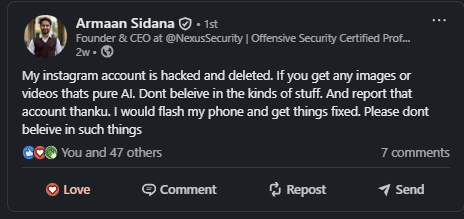
\includegraphics[width=0.8\textwidth]{1.png}}
    \caption{Armaan Sidana explaining that his Instagram account got hacked}
\end{figure}

\section*{Example 2: Faiyaz Ahmad}

Faiyaz Ahmad is a recognized bug bounty hunter and YouTuber with over 33,000 subscribers on his channel \textit{BePracticalTech}. On August 11, 2025, his official Telegram Messenger channel was hacked. The hacker used it to promote scams and gambling apps under his name, putting thousands of people at risk.

\begin{figure}[H]
    \centering
    \fbox{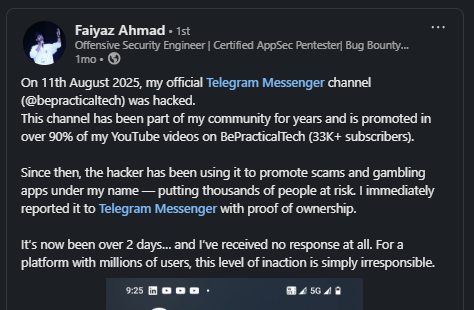
\includegraphics[width=0.8\textwidth]{2.png}}
    \caption{Faiyaz Ahmad sharing how his Telegram channel was hacked}
\end{figure}

\section*{Why Famous People Are Easy Targets for Social Engineering}

\begin{itemize}
    \item \textbf{Multiple accounts to manage}\\
    They usually handle many platforms at once (YouTube, Instagram, Telegram, Twitter, etc.). This increases the chance of missing a security alert or phishing attempt.

    \item \textbf{Daily interactions with strangers (fans and followers)}\\
    They constantly receive messages, requests, and emails, making it hard to separate genuine fans from hackers pretending to be one.

    \item \textbf{Brand promotions and sponsorships}\\
    Hackers can pose as companies offering deals, free trials, or collaborations, which makes phishing easier.

    \item \textbf{High trust value}\\
    Anything shared from their account is trusted by thousands of followers, so hackers see this as a shortcut to spread scams.

    \item \textbf{Busy schedules}\\
    Being active in business, content creation, and social life leaves them with less time to carefully check every link or attachment.

    \item \textbf{Publicly available information}\\
    A lot of their personal or professional details are online, making it easier for attackers to craft convincing phishing messages.
\end{itemize}

\section*{Conclusion}

Famous people face more risk of being hacked not because they lack technical knowledge, but because their visibility makes them attractive targets. Hackers know that compromising one account of a well-known person can cause bigger impact than targeting a random individual. This is why awareness, strict security practices, and multi-factor authentication are critical for them.

\end{document}